\documentclass[border=2pt]{standalone}
\usepackage{tikz}
\usetikzlibrary{matrix,positioning,arrows.meta,arrows,calc}
\begin{document}
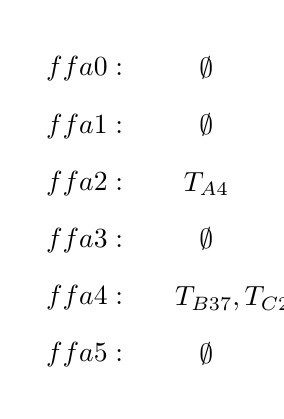
\begin{tikzpicture}[>=latex]

\tikzset{
mymat/.style={
  matrix of math nodes,
  text height=2.5ex,
  text depth=0.75ex,
  text width=5.25ex,
  align=center,
  column sep=-\pgflinewidth
},
mymats/.style={
  mymat,
  text width=8ex,
  nodes={draw} 
}}

\matrix[mymat,anchor=north]
at (0,0) 
(mat1)
{
ffa0:\\
ffa1:\\
ffa2:\\
ffa3:\\
ffa4:\\
ffa5:\\
};

\matrix[mymat,anchor=west]
at (1,-6.6em) 
(mat2)
{
\emptyset\\
\emptyset\\
T_{A4}\\
\emptyset\\
T_{B37}, T_{C2}\\
\emptyset\\
};



\end{tikzpicture}
\end{document}